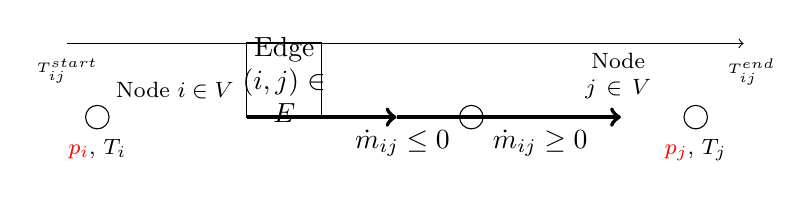
\begin{tikzpicture}[scale=.95]
    \draw[fill=white] (3,0) rectangle (4,1);
    \node[text width=1.2cm,align=center] at (3.5,.5) {Edge $(i,j)\in E$};
    \draw[->,line width=1.5pt] (3,0)--(5,0);
    \draw[line width=1.5pt] (5,0)--(7,0);
    \draw[->,line width=1.5pt] (7,0)--(8,0);
    \node[circle,draw,inner sep=3pt,label=-15:$\dot{m}_{ij}\geq 0$,label=-165:$\dot{m}_{ij}\leq 0$,font=\footnotesize,anchor=center] at (6,0) {};

    \begin{scope}[local bounding box=scope]
        \node[circle,draw,inner sep=3pt,label={[font=\footnotesize,text width=1.5cm,align=center]above right:{Node $i\in V$}},label={[font=\footnotesize,align=center]below:{\textcolor{red}{$p_i$}, {$T_i$}}}] at (1,0) {};
        \node[circle,draw,inner sep=3pt,label={[font=\footnotesize,text width=1.5cm,align=center]above left:{Node $j\in V$}},label={[font=\footnotesize,align=center]below:{\textcolor{red}{$p_j$}, {$T_j$}}}] at (9,0) {};
        \draw[->] ([xshift=3pt]scope.north west)--([xshift=3pt]scope.north east);
        \node[below=2pt] at ([xshift=3pt]scope.north west) {\tiny{$T_{ij}^{start}$}};
        \node[below=2pt] at ([xshift=3pt]scope.north east) {\tiny{$T_{ij}^{end}$}};
    \end{scope}
\end{tikzpicture}